\documentclass[11pt,a4paper]{article}

% --- Common Packages across layouts --- %\
\usepackage{lmodern} % Required before microtype to prevent erroring.
\usepackage{microtype}
\usepackage{graphicx}
\usepackage[hidelinks]{hyperref}
\usepackage{xcolor}
\usepackage{todonotes}
\usepackage{dirtytalk}
\usepackage{siunitx}
\usepackage{xspace}
\usepackage{fontawesome5}
\usepackage{lipsum} % For testing

%\usepackage{allrunes} package allrunes to add, but currently unstable due to trying to redefine \swdefault and \dot



% Article and report specific packages %

% Visual style packages

\usepackage[margin = 4cm]{geometry}
\usepackage{wrapfig}
\usepackage{caption}
\usepackage{subcaption}
\usepackage[nocheck]{fancyhdr}
\usepackage{titlesec}
\usepackage{blindtext}
\usepackage{enumitem}
\setitemize{itemsep=2pt, topsep=4pt, parsep=4pt, partopsep=6pt}

% Maths / Science packages
\usepackage{amsfonts, amssymb, amsmath, amsthm}
\usepackage{bm}
\usepackage{physics}
\usepackage{tikz}
\usepackage{circuitikz}
\usepackage{cancel}
\usepackage{mathrsfs} % New font family from \mathscr{}, \mathfrak{}.

% Other utility packages
\usepackage{multicol}
\usepackage{afterpage}
\usepackage[backend=biber, style=numeric]{biblatex}
\addbibresource{references.bib}



% My (John's) personal utility packages
\usepackage{packages/johns-package-setup}
\usepackage{packages/johns-preferences}


% ============================================ %
%    ARTICLE / SHORT REPORT TEMPLATE         %
% ============================================ %

% Article/short report template specific tweaks -- consider turning into a new (conditional) package
\numberwithin{equation}{section}

% Setting up headers and footers for fancyhf
\fancyhf{}
\fancyhead[R]{\today}
\fancyhead[L]{Keyboard Layout}
\fancyfoot[C]{\thepage}
\headsep = 15pt
\voffset = 10pt

% Title and introduction to the report
\title{Keyboard Layout}
\author{John Perry\thanks{Churchill College}}
\date{\today}

\begin{document}

\pagestyle{empty}
\newgeometry{margin = 3cm}
\pagenumbering{arabic}

\maketitle

% Set headers and footers to exist past the title page
% \afterpage{\thispagestyle{fancy}} % Was useful when not dealing with multicol
\pagestyle{fancy}


\begin{abstract}
    % Give the abstract of the document with the reason it exists, the significance of its contribution to the project and the conclusions it provides.
    This document contains more detailed discussion of the layout of the keyboard, with a visual example of how the layout changes over time.
\end{abstract}

\section{Introduction}
% Introduce the problem, and contextualise it and the objectives of the experiment/thing being reported on

The goals for the keyboard and keyboard layout as a whole is to provide a medium to control all aspects of a GUI-focused system with a focus on coding. The main goal is to keep a close-enough similarity to \textsc{QWERTY}, without any of the most agregious annoyances when it comes to coding---such as some of the locations of bracket and special keys---enabling a more fluid experience.

\section{Visual Layout}

\begin{figure}[h]
    \centering
    \begin{subfigure}{0.495\textwidth}
        \centering
        \begin{tikzpicture}[line width=0.8pt, black, scale=0.95]
            % Draw the 7x5 grid
            \draw (0,0) grid (6,5);
            
            \draw[ultra thick] (0,0) -- (0,5) -- (6,5) -- (6,0) -- (0,0);

            \draw[ultra thick, red] (1,2) -- (1,3) -- (5,3) -- (5,2) -- (1,2);

            % Draw the extra section for potential pop-out Steam Deck trackpads
            \draw[ultra thick] (6,1) -- (8,-1) -- (6.6,-2.4) -- (4,0);

            % Draw in the rows of symbols for the main symbol
            \foreach \x in {0.35} {
                \foreach \y in {0.25} {
                    \node at (\x, \y + 4) {esc};
                    \node at (\x + 1, \y + 4) {1};
                    \node at (\x + 2, \y + 4) {2};
                    \node at (\x + 3, \y + 4) {3};
                    \node at (\x + 4, \y + 4) {4};
                    \node at (\x + 5, \y + 4) {5};

                    \node at (\x, \y + 3) {tab};
                    \node at (\x + 1, \y + 3) {Q};
                    \node at (\x + 2, \y + 3) {W};
                    \node at (\x + 3, \y + 3) {E};
                    \node at (\x + 4, \y + 3) {R};
                    \node at (\x + 5, \y + 3) {T};

                    \node at (\x, \y + 2) {caps};
                    \node at (\x + 1, \y + 2) {A};
                    \node at (\x + 2, \y + 2) {S};
                    \node at (\x + 3, \y + 2) {D};
                    \node at (\x + 4, \y + 2) {F};
                    \node at (\x + 5, \y + 2) {G};

                    \node at (\x, \y + 1) {shift};
                    \node at (\x + 1, \y + 1) {Z};
                    \node at (\x + 2, \y + 1) {X};
                    \node at (\x + 3, \y + 1) {C};
                    \node at (\x + 4, \y + 1) {V};
                    \node at (\x + 5, \y + 1) {B};

                    \node at (\x, \y) {ctrl};
                    \node at (\x + 1, \y) {\faWindows};
                    \node at (\x + 2, \y) {alt};
                    \node at (\x + 3, \y) {$($};
                    \node at (\x + 4, \y) {fn};
                    \node at (\x + 5, \y) {\rotatebox[origin=c]{180}{\Large{$\Rsh$}}};
                }
            }

            \foreach \x in {0.3} {
                \foreach \y in {0.75} {
                    \node at (\x, \y + 4) {};
                    \node at (\x + 1, \y + 4) {};
                    \node at (\x + 2, \y + 4) {};
                    \node at (\x + 3, \y + 4) {};
                    \node at (\x + 4, \y + 4) {};
                    \node at (\x + 5, \y + 4) {};

                    \node at (\x, \y + 3) {};
                    \node at (\x + 1, \y + 3) {};
                    \node at (\x + 2, \y + 3) {};
                    \node at (\x + 3, \y + 3) {};
                    \node at (\x + 4, \y + 3) {};
                    \node at (\x + 5, \y + 3) {};

                    \node at (\x, \y + 2) {};
                    \node at (\x + 1, \y + 2) {};
                    \node at (\x + 2, \y + 2) {};
                    \node at (\x + 3, \y + 2) {};
                    \node at (\x + 4, \y + 2) {};
                    \node at (\x + 5, \y + 2) {};

                    \node at (\x, \y + 1) {};
                    \node at (\x + 1, \y + 1) {};
                    \node at (\x + 2, \y + 1) {};
                    \node at (\x + 3, \y + 1) {};
                    \node at (\x + 4, \y + 1) {};
                    \node at (\x + 5, \y + 1) {};

                    \node at (\x, \y) {};
                    \node at (\x + 1, \y) {};
                    \node at (\x + 2, \y) {};
                    \node at (\x + 3, \y) {$[$};
                    \node at (\x + 4, \y) {};
                    \node at (\x + 5, \y) {\Huge{␣}};
                }
            }

            \foreach \x in {0.7} {
                \foreach \y in {0.75} {
                    \node at (\x, \y + 4) {};
                    \node at (\x + 1, \y + 4) {\small{F1}};
                    \node at (\x + 2, \y + 4) {\small{F2}};
                    \node at (\x + 3, \y + 4) {\small{F3}};
                    \node at (\x + 4, \y + 4) {\small{F4}};
                    \node at (\x + 5, \y + 4) {\small{F5}};

                    \node at (\x, \y + 3) {};
                    \node at (\x + 1, \y + 3) {};
                    \node at (\x + 2, \y + 3) {};
                    \node at (\x + 3, \y + 3) {};
                    \node at (\x + 4, \y + 3) {};
                    \node at (\x + 5, \y + 3) {};

                    \node at (\x, \y + 2) {};
                    \node at (\x + 1, \y + 2) {};
                    \node at (\x + 2, \y + 2) {};
                    \node at (\x + 3, \y + 2) {};
                    \node at (\x + 4, \y + 2) {};
                    \node at (\x + 5, \y + 2) {};

                    \node at (\x, \y + 1) {};
                    \node at (\x + 1, \y + 1) {};
                    \node at (\x + 2, \y + 1) {};
                    \node at (\x + 3, \y + 1) {};
                    \node at (\x + 3.9, \y + 1) {\tiny{home}};
                    \node at (\x + 4.9, \y + 1) {\tiny{pg.up}};

                    \node at (\x, \y) {};
                    \node at (\x + 1, \y) {};
                    \node at (\x + 2, \y) {};
                    \node at (\x + 3, \y) {$\{$};
                    \node at (\x + 4, \y) {};
                    \node at (\x + 5, \y) {};
                }
            }
        \end{tikzpicture}
        \caption{Left Hand}\label{fig:left-hand-layout}
    \end{subfigure}
    \begin{subfigure}{0.495\textwidth}
        \centering
        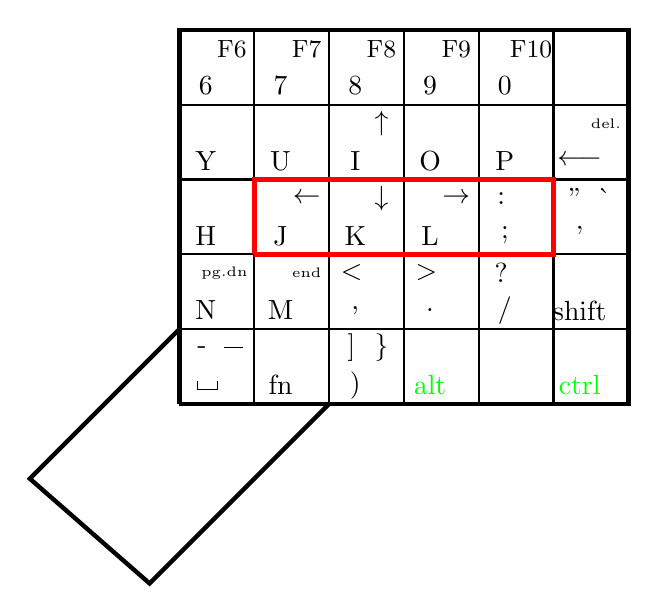
\begin{tikzpicture}[line width=0.8pt, black, scale=0.95]
            % Draw the 7x5 grid
            \draw (0,0) grid (6,5);
            
            \draw[ultra thick] (0,0) -- (0,5) -- (6,5) -- (6,0) -- (0,0);

            \draw[ultra thick, red] (1,2) -- (1,3) -- (5,3) -- (5,2) -- (1,2);

            % Draw the extra section for potential pop-out Steam Deck trackpads
            \draw[ultra thick] (0,1) -- (-2,-1) -- (-0.4,-2.4) -- (2,0);

            % Draw in the rows of symbols for the main symbol
            \foreach \x in {0.35} {
                \foreach \y in {0.25} {
                    \node at (\x, \y + 4) {6};
                    \node at (\x + 1, \y + 4) {7};
                    \node at (\x + 2, \y + 4) {8};
                    \node at (\x + 3, \y + 4) {9};
                    \node at (\x + 4, \y + 4) {0};
                    \node at (\x + 5, \y + 4) {};

                    \node at (\x, \y + 3) {Y};
                    \node at (\x + 1, \y + 3) {U};
                    \node at (\x + 2, \y + 3) {I};
                    \node at (\x + 3, \y + 3) {O};
                    \node at (\x + 4, \y + 3) {P};
                    \node at (\x + 5, \y + 3) {$\longleftarrow$};

                    \node at (\x, \y + 2) {H};
                    \node at (\x + 1, \y + 2) {J};
                    \node at (\x + 2, \y + 2) {K};
                    \node at (\x + 3, \y + 2) {L};
                    \node at (\x + 4, \y + 2) {;};
                    \node at (\x + 5, \y + 2) {'};

                    \node at (\x, \y + 1) {N};
                    \node at (\x + 1, \y + 1) {M};
                    \node at (\x + 2, \y + 1) {,};
                    \node at (\x + 3, \y + 1) {.};
                    \node at (\x + 4, \y + 1) {/};
                    \node at (\x + 5, \y + 1) {shift};

                    \node at (\x, \y) {\Huge{␣}};
                    \node at (\x + 1, \y) {fn};
                    \node at (\x + 2, \y) {$)$};
                    \node at (\x + 3, \y) {\textcolor{green}{alt}};
                    \node at (\x + 4, \y) {};
                    \node at (\x + 5, \y) {\textcolor{green}{ctrl}};
                }
            }

            \foreach \x in {0.3} {
                \foreach \y in {0.75} {
                    \node at (\x, \y + 4) {};
                    \node at (\x + 1, \y + 4) {};
                    \node at (\x + 2, \y + 4) {};
                    \node at (\x + 3, \y + 4) {};
                    \node at (\x + 4, \y + 4) {};
                    \node at (\x + 5, \y + 4) {};

                    \node at (\x, \y + 3) {};
                    \node at (\x + 1, \y + 3) {};
                    \node at (\x + 2, \y + 3) {};
                    \node at (\x + 3, \y + 3) {};
                    \node at (\x + 4, \y + 3) {};
                    \node at (\x + 5, \y + 3) {};

                    \node at (\x, \y + 2) {};
                    \node at (\x + 1, \y + 2) {};
                    \node at (\x + 2, \y + 2) {};
                    \node at (\x + 3, \y + 2) {};
                    \node at (\x + 4, \y + 2) {:};
                    \node at (\x + 5, \y + 2) {"};

                    \node at (\x, \y + 1) {};
                    \node at (\x + 1, \y + 1) {};
                    \node at (\x + 2, \y + 1) {$<$};
                    \node at (\x + 3, \y + 1) {$>$};
                    \node at (\x + 4, \y + 1) {?};
                    \node at (\x + 5, \y + 1) {};

                    \node at (\x, \y) {-};
                    \node at (\x + 1, \y) {};
                    \node at (\x + 2, \y) {]};
                    \node at (\x + 3, \y) {};
                    \node at (\x + 4, \y) {};
                    \node at (\x + 5, \y) {};
                }
            }

            \foreach \x in {0.7} {
                \foreach \y in {0.75} {
                    \node at (\x, \y + 4) {\small{F6}};
                    \node at (\x + 1, \y + 4) {\small{F7}};
                    \node at (\x + 2, \y + 4) {\small{F8}};
                    \node at (\x + 3, \y + 4) {\small{F9}};
                    \node at (\x + 4, \y + 4) {\small{F10}};
                    \node at (\x + 5, \y + 4) {};

                    \node at (\x, \y + 3) {};
                    \node at (\x + 1, \y + 3) {};
                    \node at (\x + 2, \y + 3) {$\uparrow$};
                    \node at (\x + 3, \y + 3) {};
                    \node at (\x + 4, \y + 3) {};
                    \node at (\x + 5, \y + 3) {\tiny{del.}};

                    \node at (\x, \y + 2) {};
                    \node at (\x + 1, \y + 2) {$\leftarrow$};
                    \node at (\x + 2, \y + 2) {$\downarrow$};
                    \node at (\x + 3, \y + 2) {$\rightarrow$};
                    \node at (\x + 4, \y + 2) {};
                    \node at (\x + 5, \y + 2) {\textasciigrave};

                    \node at (\x - 0.1, \y + 1) {\tiny{pg.dn}};
                    \node at (\x + 1, \y + 1) {\tiny{end}};
                    \node at (\x + 2, \y + 1) {};
                    \node at (\x + 3, \y + 1) {};
                    \node at (\x + 4, \y + 1) {};
                    \node at (\x + 5, \y + 1) {};

                    \node at (\x, \y) {\Huge{\_}};
                    \node at (\x + 1, \y) {};
                    \node at (\x + 2, \y) {$\}$};
                    \node at (\x + 3, \y) {};
                    \node at (\x + 4, \y) {};
                    \node at (\x + 5, \y) {};
                }
            }
        \end{tikzpicture}
        \caption{Right Hand}\label{fig:right-hand-layout}
    \end{subfigure}
    \caption{Hand layouts for the proposed keyboard layout. Potential \href{https://www.steamdeck.com/en/tech}{Steam Deck trackpads} are shown approximately where the thumbs come out. Elements in green are mappings that are not fully confident.}\label{fig:proposed-keyboard-layout}
\end{figure}

\subsection{Notes on the layout}

A few notes on some things to note with the keyboard layout in Figure~\ref{fig:proposed-keyboard-layout}:
\begin{itemize}
    \item The space key on the left side of the keyboard is partially illustrative of the fact that it should still operate as a \say{jump} button with games.
\end{itemize}

\end{document}

